\chapter{Исследование взаимодействия имплантируемого роторного насоса крови и сердечно-сосудистой системы с использованием экспериментальных данных для роторных насосов крови Спутник} \label{chapt4}

Цель данной главы заключается в исследовании взаимодействия имплантируемого роторного насоса крови и сердечно-сосудистой системы с использованием экспериментальных данных для имплантируемых роторных насосов крови Спутник. % 

\section{Анализ исходных данных}

Фотографии имплантируемых роторных насосов крови Спутник первого и второго поколений -- далее Спутник 1 и Спутник 2 -- представлены на рисунке \ref{img:sputnik_pumps}. Описание насосов приведено в разделе \ref{chapt1_irbps}.

% \begin{figure}[ht]
%   \center{\includegraphics [scale=0.50] {../images/c5_Sputniks}}
% %   \begin{minipage}[ht]{0.49\linewidth}
% %     \center{\includegraphics [scale=1.0] {../images/c5_sputnik_1} \\ а)}
% %   \end{minipage}
% %   \hfill
% %   \begin{minipage}[ht]{0.49\linewidth}
% %     \center{\includegraphics [scale=0.93] {../images/c5_sputnik_2} \\ б)}
% %   \end{minipage}
%   \caption{Первое поколение (слева) и второе поколение (справа) имплантируемого роторного насоса крови <<Спутник>>}
%   \label{img:sputnik_pumps}  
% \end{figure}

% Первое поколение РНК на данный момент применяется в клинических условиях \cite{selishchev2015ventricular} -- общее количество имплантаций более тридцати раз. По сравнению с насосом первого поколения масса насоса второго поколения РНК уменьшена с 246 г до 205 г, энергопотребление на 15\% \cite{sputnik_upd}. В настоящий момент второе поколение РНК находится на этапе \textit{in vivo} испытаний. 

Экспериментальное исследование насосов проведено в испытательном гидродинамическом стенде, расположенном в Институте Гельмгольца по биомедицинской инженерии (г. Ахен, Германия) \cite{Misgeld201535,heinke_modeling_2015}. Схема гидродинамического стенда представлена на рисунке \ref{img:mcl}а. Система управления стендом с помощью специальных приводных механизмов формировала давления в камерах $C_{in}$ и $C_{out}$, что позволяло создать перепад давления в системе аналогично сердечно-сосудистой системе.

%\begin{figure}[!ht] 
%  \center
 % \includegraphics [scale=1.8] {../images/mcl_scheme}
%  \caption{Схема испытательного гидродинамического стенда} 
 % \label{img:mcl}  
%\end{figure}

\begin{figure}[!ht]
  \begin{minipage}[ht]{0.55\linewidth}
    \center{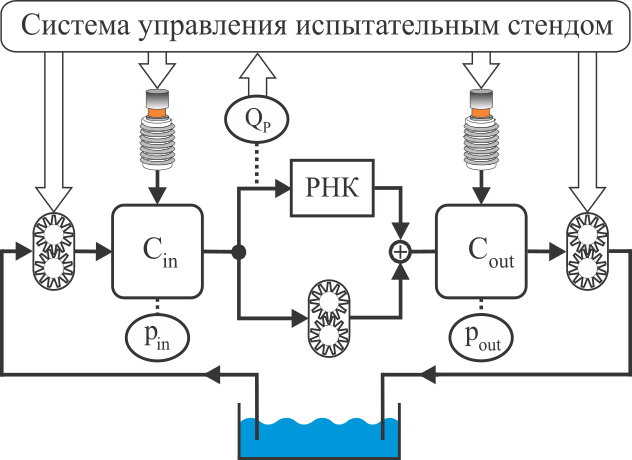
\includegraphics[scale=1.45]{../images/c4_mcl_scheme} \\ а)}
  \end{minipage}
  \hfill
  \begin{minipage}[ht]{0.44\linewidth}
    \center{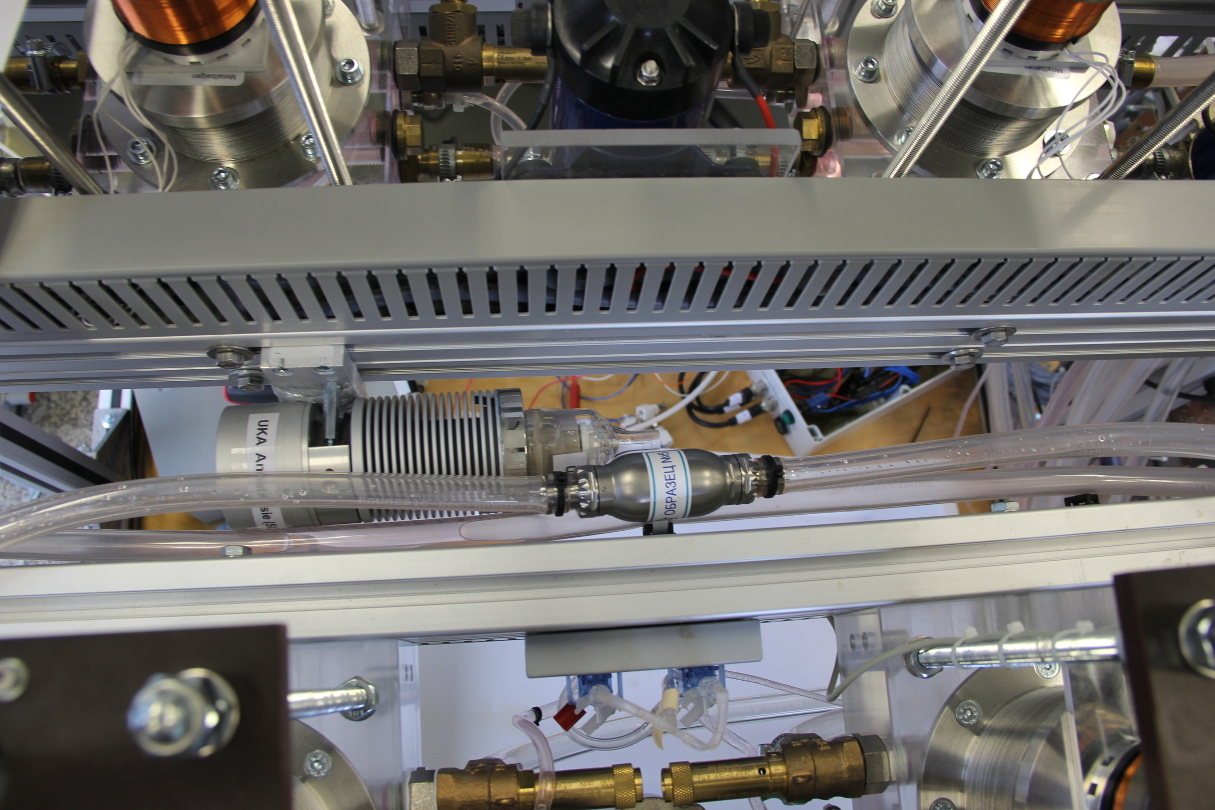
\includegraphics[scale=0.16]{../images/c4_mcl_photo} \\ б)}
  \end{minipage}
  \caption{Схема испытательного гидродинамического стенда (а) и фото в момент проведения испытаний (б)}
  \label{img:mcl}  
\end{figure}

Вязкость жидкости в контуре гидродинамического стенда равнялась 2,5 сП, частота сердечных сокращений -- 80 уд/мин. В стенде последовательно воспроизводились два состояния сердечно-сосудистой системы, соответствующие различным степеням сердечной недостаточности. Данные состояния были воспроизведены посредством задания физиологического параметра contractilityFactor (cF) равным 0,5 и 0,25, где cF равное 1 соответствует нормальной функции сердца.

Расход насоса регистрировался ультразвуковым датчиком (H11XL, Transonic Systems Inc., Ithaca, США). Измерение давлений на входе и выходе насоса производилось посредством датчиков давлений (Xtrans, CODAN pvb Critical Care GmbH Forstinning, Германия). Управление работой насосов осуществлялось с помощью программного обеспечения ESCON Studio и контроллера ESCON Module 50/54 EC-S (Maxon Motor AG, Швейцария).

% Первоначальные исследования проведены в статических условиях. С помощью системы управления стендом на насосе фиксировался постоянный перепад давления после чего регистрировался расход насоса. Перепад давления изменялся в диапазоне от -50 мм рт. ст. до 150 мм рт. ст. с шагом 25 мм рт. ст., скорость вращения ротора насоса изменялась от 5000 об/мин до 10000 об/мин с шагом 1000 об/мин.
% 
% Результаты исследования представлены на рисунке \ref{img:static_HQ_sputnik}. Полученные характеристики демонстрируют отличия в производительности исследованных роторных насосов крови. 
% 
% \begin{figure}[ht] 
%   \center
%   \includegraphics [scale=1.0] {../images/c5_static_hq}
%   \caption{Статические расходно-напорные характеристики роторных насосов крови Спутник 1 (слева) и Спутник 2 (справа) при различных скоростях насоса} 
%   \label{img:static_HQ_sputnik}  
% \end{figure}
% 
% После этого были проведены исследования в динамических условиях. Результаты получены в состояниях, соответствующих различным степеням сердечной недостаточности. Данные состояние были вопроизведены посредством задания параметра contractilityFactor (cF) равным 0,5 и 0,25, где cF равное 1 соответствует нормальной функции желудочка сердца. 

Скорость вращения ротора насоса изменялась в диапазоне от 5000 до 10000 об/мин с шагом 200 об/мин. На каждом шаге в течение примерно 30 секунд записывались временные диаграммы расхода насоса, скорости вращения ротора, давления на входе и на выходе насоса и потока через аортальный клапан. %Расходно-напорные характеристики имплантируемых роторных насосов крови <<Спутник>> и циклические зависимости давления от объема желудочка сердца представлены на рисунках \ref{img:experimental_results_S1} и \ref{img:experimental_results_S2}.

% \begin{figure}
%   \center
%   \includegraphics[scale=1.0]{../images/pv_hq_05_025}
%   \caption{Расходно-напорные характеристики насоса Спутник 1 (сверху) и соответствующие циклические зависимости давления от объема левого желудочка сердца (снизу) в состояниях cF 0,5 (слева) cF 0,25 (справа) в диапазоне скоростей от 5000 об/мин (\textcolor{blue}{\rule[0.8 mm]{3 mm}{.55pt}}) \\ до 9000 об/мин (\textcolor{blue}{\rule[0.6 mm]{3 mm}{1.2pt}})} 
%   \label{img:experimental_results_S1}
% \end{figure}
% 
% \begin{figure}
%   \center
%   \includegraphics[scale=1.0]{../images/pv_hq_05_025_S2}
%   \caption{Расходно-напорные характеристики насоса Спутник 2 (сверху) и соответствующие циклические зависимости давления от объема левого желудочка сердца (снизу) в состояниях cF 0,5 (слева) cF 0,25 (справа) в диапазоне скоростей от 5000 об/мин (\textcolor{blue}{\rule[0.8 mm]{3 mm}{.55pt}}) \\ до 9000 об/мин (\textcolor{blue}{\rule[0.6 mm]{3 mm}{1.2pt}})} 
%   \label{img:experimental_results_S2}
% \end{figure}

В ходе анализа экспериментальных данных не удалось выявить режимы частичного коллапса и полного коллапса желудочка сердца. В качестве замены был предложен режим коллапса желудочка сердца $P_{VC}$, определяемый как отрицательное конечно-диастолического давление в желудочке сердца. %Величина давления для каждой скорости вращения ротора вычислялось как среднее значение за 25 сердечных циклов.

Режимы частичной разгрузки и полной разгрузки желудочка сердца определялись как наличие и отсутствие потока через аортальный клапан. %Поток через аортальный клапан для каждой скорости вращения ротора насоса вычислялся как интегральный поток в течение 20 секунд.

Режим обратного течения через насос определялся как отрицательный расход во временной диаграмме расхода насоса. %Минимальная величина расхода насоса за время сердечного цикла для каждой скорости вращения ротора вычислялась как среднее значение за 25 сердечных циклов. 

Таким образом в данной главе рассматриваются четыре режима работы имплантируемого роторного насоса крови: режим обратного течения через насос $P_{BF}$, режим частичной разгрузки $P_{PA}$, режим полной разгрузки желудочка сердца $P_{FA}$ и режим коллапса желудочка сердца $P_{VC}$. Данные режимы работы представлены с помощью гемодинамических зависимостей на рисунке \ref{img:ps_sputnik_1} для насоса Спутник 1 и на рисунке \ref{img:ps_sputnik_2} для насоса Спутник 2. Маркерами отмечены переходы между режимами работы насоса аналогично рисунку \ref{img:pumping_states_general}. 

\begin{figure}[!ht] 
  \center
  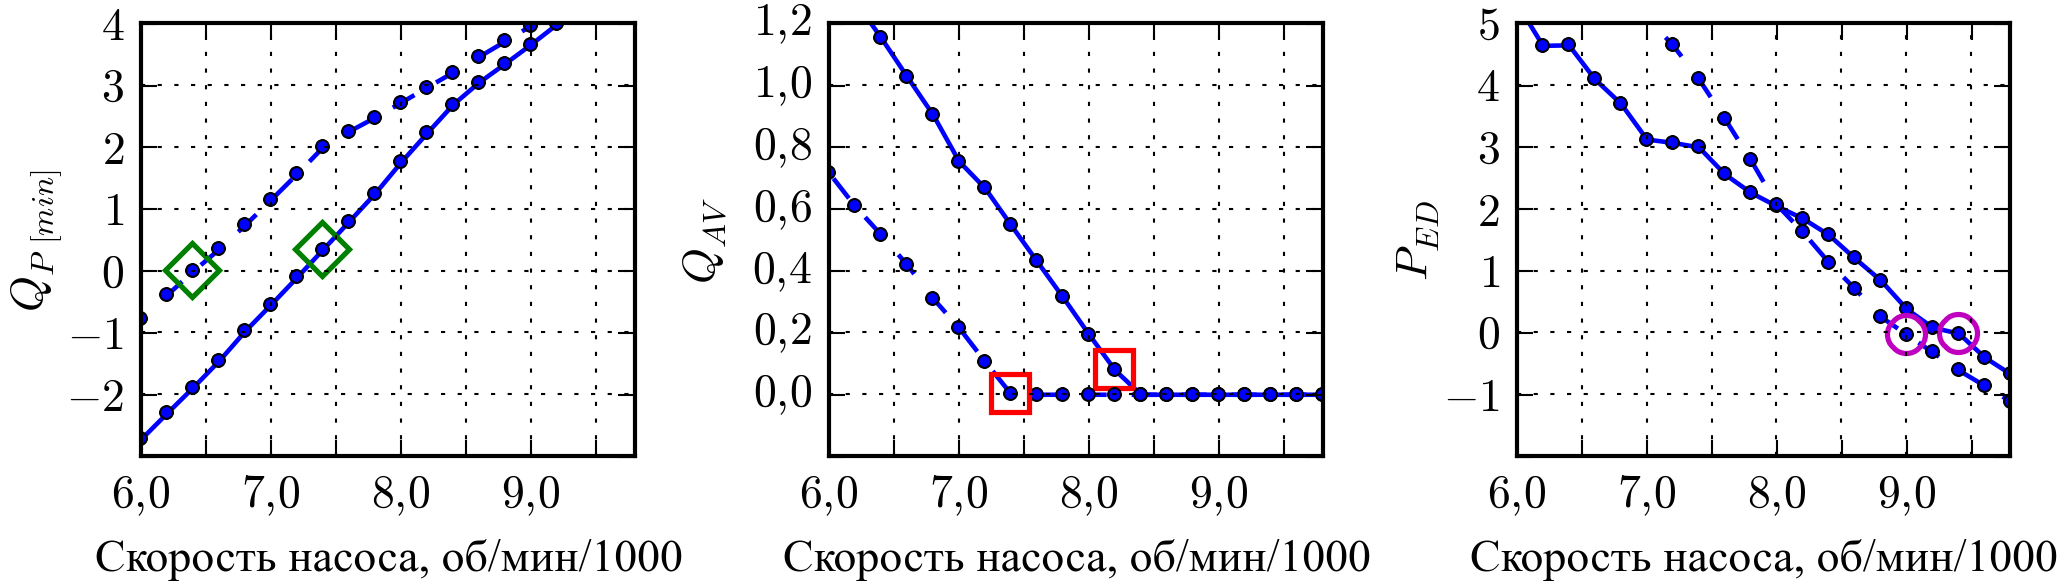
\includegraphics [scale=1.0] {../images/c4_ps_sputnik_1}
  \caption{Изменения в гемодинамике в состояниях cF 0,5 (сплошная линия) и cF 0,25 (пунктирная линия) для насоса Спутник 1; $Q_{P[min]}$ -- минимальный расход насоса во время сердечного цикла (л/мин), $Q_{AV}$ -- объемный поток через аортальный клапан (л), $P_{ED}$ -- конечно-диастолическое давление желудочка сердца (мм рт. ст.)} 
  \label{img:ps_sputnik_1}  
\end{figure}

\begin{figure}[!ht] 
  \center
  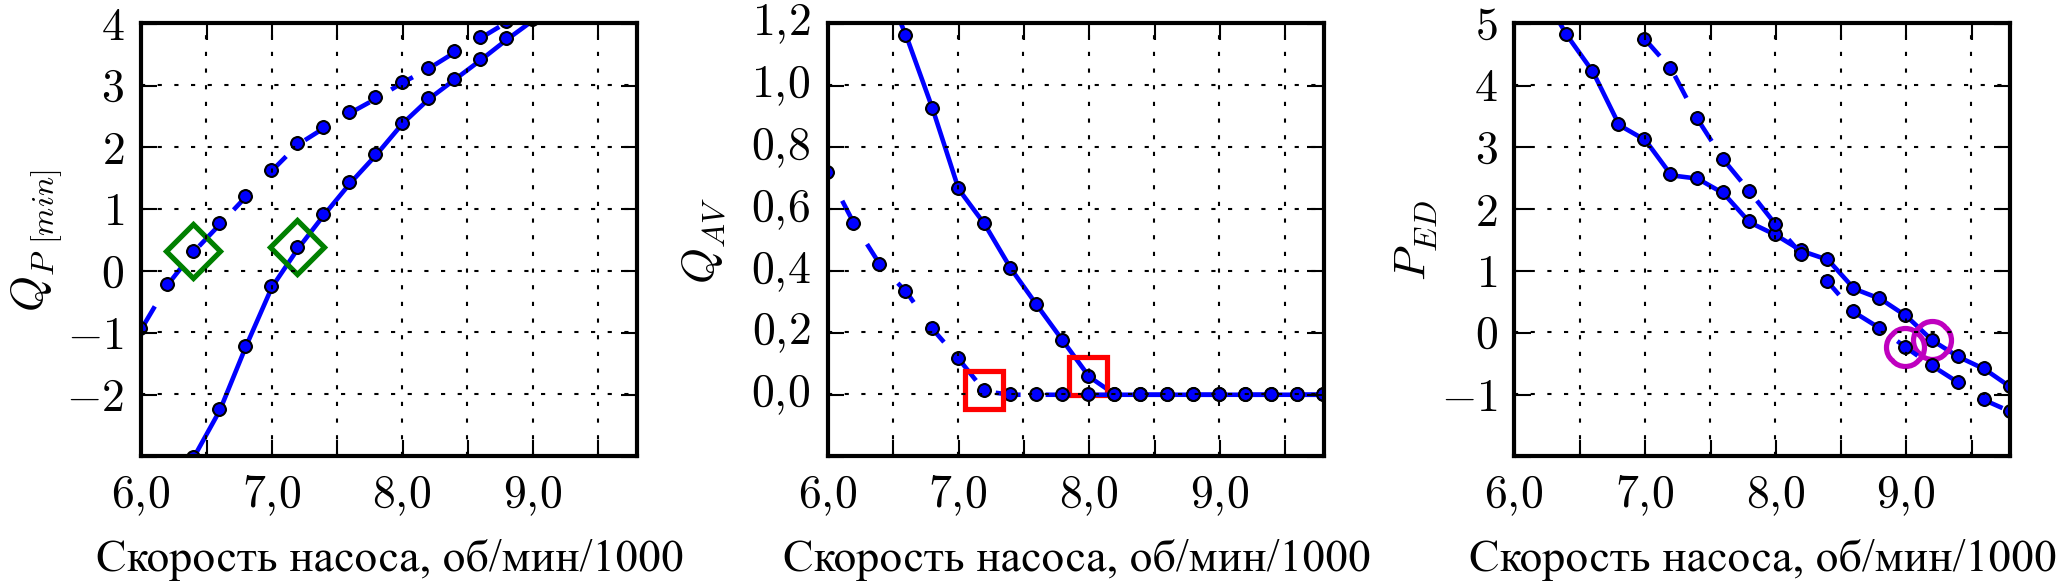
\includegraphics [scale=1.0] {../images/c4_ps_sputnik_2}
  \caption{Изменения в гемодинамике в состояниях cF 0,5 (сплошная линия) и cF 0,25 (пунктирная линия) для насоса Спутник 2; $Q_{P[min]}$ -- минимальный расход насоса во время сердечного цикла (л/мин), $Q_{AV}$ -- объемный поток через аортальный клапан (л), $P_{ED}$ -- конечно-диастолическое давление желудочка сердца (мм рт. ст.)} 
  \label{img:ps_sputnik_2}  
\end{figure}

Результаты анализа полученных экспериментальных данных представлены на 44-й конференции европейского сообщества по искусственным органам \cite{esao_2017}.

На основе полученных экспериментальных данных проведено исследование характеристик имплантируемого роторного насоса крови Спутник 1, которое опубликовано в журнале <<Медицинская техника>> \cite{mt6_2015, mt6_2016}.

%в работе \cite{mt6_2015} и на конференциях \cite{asaio_2016, isrbp_2016, esao_2017}.

% ----------------------------------------------------------------------------------------------------------------------------------------------------------------------------------------------------------------------------
% ----------------------------------------------------------------------------------------------------------------------------------------------------------------------------------------------------------------------------

\section{Идентификация роторных насосов крови Спутник}

В \ref{chapt3}-й главе были предложены критерии для оценки эффективности идентификации: точность оценки расхода насоса и точность определения перехода между режимами работы насоса. В данной главе были введены следующие пороговые величины для данных критериев: средняя точность оценки расхода насоса не менее 90\%, точность определения переходов между режимами работы насоса не менее 80\%.

Точность оценки расхода насоса для каждой скорости вращения ротора рассчитывалась по формуле:

\begin{equation}
	\left( 1 - (Q_M - Q_E)/Q_M \right) \cdot 100 \%,
\end{equation}

\noindent где $Q_M$ -- интегрированное значение расхода насоса, измеренного датчиком за время равное 20 секунд, $Q_E$ -- интегрированное значение расхода насоса, вычисленного с помощью математической модели в аналогичном временном диапазоне.  

Точность определения режимов работы насоса рассчитывалась по формуле \eqref{eq:ps_identification_accuracy}. Зависимости, продемонстрированные на рисунках \ref{img:ps_sputnik_1} и \ref{img:ps_sputnik_2} позволяют определить $\omega_{max}$ и $\omega_{min}$ аналогично разделу \ref{sect3_3}. Для насоса Спутник 1 $\omega_{max}$ и $\omega_{min}$ равны 9600 об/мин и 7200 об/мин соответственно, для насоса Спутник 2 -- 9400 об/мин и 7000 об/мин.

Первоначально для описания имплантируемых роторных насосов крови Спутник использовано уравнение\eqref{eq:initial_eq}, из которого был исключен параметр $\mu$, характеризующий вязкость жидкости:

\begin{equation}
	\label{eq:initial_dynamic}
	L\frac{dQ}{dt} = aQ + b\omega^2 + cH.
\end{equation}

Коэффициенты уравнения \eqref{eq:initial_dynamic} были определены для каждого роторного насоса крови с помощью разработанной процедуры оптимизации на основе алгоритма дифференциальной эволюции \cite{storn1997differential,price2006differential}. Входными параметрами для уравнения выбраны измеренные не подвергнутые обработке временные диаграммы перепада давления в насосе и скорости вращения ротора насоса продолжительностью 1,5 секунды, полученные в состоянии cF 0,5 в диапазоне скоростей от 5800 об/мин до 9800 об/мин с шагом 400 об/мин. Процедура оптимизации реализована на языке Python с использованием библиотек NumPy и SciPy. Программный код процедуры приведен в приложении \ref{list:optimization_routine_diff}. 

Установлено, что с математической моделью, описываемой уравнением \eqref{eq:initial_dynamic}, средняя точность оценки расхода для насоса Спутник 1 составила 84,7\%, для насоса Спутник 2 -- 72,3\%. Средняя точность определения режима $P_{BF}$ для обоих насосов не превысила 70\%, точность определения режимов частичной и полной разгрузки желудочка для Спутник 2 составила менее 75\%, а точность определения $P_{VC}$ для Спутник 1 -- не более 80\%. 

Аналогичным образом проведено исследование разработанной математической модели, описываемой уравнением \eqref{eq:final_pump_model}. Установлено, что средняя точность оценки расхода для насоса Спутник 1 составила 97,6\%, для насоса Спутник 2 -- 82,5\%, точность определения перехода $P_{FA}/P_{VC}$ не превысила 75\% для обоих насосов. 

% После оптимизации уравнения \eqref{eq:initial_dynamic} для каждого роторного насоса выполнен расчет средней точности оценки расхода насоса и точности определения переходов между режимами работы насоса. Установлено, что 

Таким образом, уравнения \eqref{eq:initial_dynamic} и уравнение \eqref{eq:final_pump_model} не позволяют достигнуть соответствия заданным пороговым величинам для критериев оценки эффективности идентификации. %Ранее разработанный алгоритм идентификации оказался неприменим к результатам описанного экспериментального исследования, что привело к модификации алгоритма. 

%\subsection{Модификация алгоритма идентификации}

Решением данной проблема стало построение математических моделей с помощью алгоритма структурно-параметрической идентификации, разработанного во \ref{chapt2}-й главе. Схема алгоритма идентификации для данного случая представлена на рисунке \ref{img:flowchart_upd}. 

 %, поскольку оно является общим для описания производительности РНК в динамических условиях согласно разделу такому-то %\ref{subsect2_2_1}.

% \begin{figure}[ht] 
%   \center
%   \includegraphics [scale=0.8] {../images/c5_algorithm}
%   \caption{Блок-схема алгоритма разработки математической модели насоса} 
%   \label{img:flowchart_development}  
% \end{figure}

\begin{figure}[!ht]
\centering
\begin{tikzpicture}[node distance=1cm, auto]  

\tikzstyle{startstop} = [rectangle, rounded corners=10pt, minimum width=3.0cm, minimum height=1.35cm,text centered, draw=black]
\tikzstyle{io} = [trapezium, trapezium left angle=70, trapezium right angle=110, minimum width=0.9cm, minimum height=1.1cm, text centered, draw=black]
\tikzstyle{process} = [rectangle, minimum width=1.1cm, minimum height=1.3cm, text centered, draw=black]
\tikzstyle{decision} = [diamond, minimum width=3.4cm, minimum height=1.35cm, text centered, draw=black]
\tikzstyle{arrow} = [thick,->,>=stealth]

\node (s) [startstop, yshift=-20.0, minimum height=0.9cm] {\parbox{4.5cm}{\small \centering Начало}};
\node (start) [process, below of=s, yshift=-20.0] {\parbox{5.95cm}{\small Задание исходного уравнения $y_i$ где $i$ -- номер итерации }};
\node (in1) [io, below of=start, yshift=-1.3cm] {\parbox{5.85cm}{\small Добавление к $y_i$ члена $k\omega^xH^yQ^z$ где $k$ -- коэффициент, $x$, $y$ и $z$ -- целые числа в диапазоне $-2 \ldots 4$}};
\node (pro1) [process, below of=in1, yshift=-2.0cm] {\parbox{7.70cm}{\small Определение коэффициентов $y_i + k\omega^xH^yQ^z$ для состояния cF 0,5 \\ Проверка соответствия критериям оценки эффективности идентификации для состояний cF 0,5 и cF 0,25}};
\node (dec1) [decision, below of=pro1, yshift=-1.60cm] {};% {\footnotesize\bf \parbox{1.5cm}{Соответствие \\ критериям}};
\node (dec2) [decision, below of=dec1, yshift=-0.8cm] {};
\node (out2a) [process, right of=dec2, yshift=0.0cm, xshift=5.2cm, minimum width=1.0cm] {\parbox{4.15cm}{\small Задание $y_i + k\omega^xH^yQ^z$ \\исходным уравнением \\ $i = i + 1$ \\ $j = j + 1$}};
\node (out2b) [io, left of=dec1, xshift=-5.3cm, minimum width=1.0cm] {\parbox{4.80cm}{\small Исключение $y_i + k\omega^xH^yQ^z$ \\ $j = j + 1$}};
\node (out2c) [process, below of=dec2, yshift=-0.8cm, minimum height=1.0cm] {\small Окончательное $y_i + k\omega^xH^yQ^z$};
\node (out) [startstop, below of=out2c, yshift=-0.5cm, minimum height=0.9cm] {\parbox{4.5cm}{\small \centering Конец}};

\draw [arrow] (s) -- (start);
\draw [arrow] (start) -- (in1);
\draw [arrow] (in1) -- (pro1);
\draw [arrow] (pro1) -- (dec1);
\draw [arrow] (out2c) -- (out);
\draw [arrow] (dec2) -- node[anchor=south] {\small нет} (out2a);
\draw [arrow] (dec1) -- node[anchor=south] {\small нет} (out2b);
\draw [arrow] (dec1) -- node[anchor=west] {\small ~да} (dec2);
\draw [arrow] (dec2) -- node[anchor=west] {\small ~да} (out2c);
\draw [arrow] (out2a) |- ($(in1.east)+(0,-0.1)$);
\draw [arrow] (out2b) |- ($(in1.west)+(0.05,0.1)$);
%\draw [arrow] (out2b) ($(out2b.east)$)|- + (2.5,0) |- ($(in1.east)+(0.05,0.1)$); 
\draw (0.0, -10.30) node {\small $\delta(Q)$ | $\delta(PS)$}; %  \\ $\delta(PS) \geq 85\%$
\draw (0.0, -12.15) node {\small $\delta(Q)$ \& $\delta(PS)$}; %  \\ $\delta(PS) \geq 85\%$
\end{tikzpicture} 
\caption{Схема алгоритма идентификации для случая идентификации роторных насосов крови Спутник} 
\label{img:flowchart_upd}  
\end{figure}

В качестве исходного выражения выбрано уравнение \eqref{eq:initial_dynamic}. Список одночленов $kx_j$ заменен членом $k\omega^xH^yQ^z$, где $k$ -- коэффициент, $x$, $y$ и $z$ -- целые числа в диапазоне от -2 до 4. На каждом шаге алгоритма $i$ осуществляется определение коэффициентов уравнения $y_i + k\omega^xH^yQ^z$ для состояния cF 0,5 и проверка на соответствие заданным пороговым величинам для состояний cF 0,5 и cF 0,25. 

Если полученное уравнение соответствует пороговым величинам для критериев оценки эффективности, то процесс построения завершается и полученное уравнение рассматривается в качестве математической модели идентификации имплантируемого роторного насоса крови. 

В случае частичного соответствия заданным пороговым величинам -- средней точности оценки расхода $\delta(Q)$ или точности определения переходов между режимами работы насоса $\delta(PS)$ -- полученное уравнение задается в качестве исходного и запускается еще один процесс оптимизации уравнения с добавлением члена $k\omega^xH^yQ^z$ и проверкой на соответствие критериям. 

В иных случаях полученное уравнение исключается из процесса идентификации. 

\subsection{Результаты идентификации}

В результате применения алгоритма структурно-параметрической идентификации построены математические модели, которые обеспечивают соответствие заданным пороговым величинам для критериев оценки эффективности идентификации. 

Математическая модель насоса Спутник 1 описывается следующим уравнением:

\begin{equation}
	\label{eq:sputnik_1_eq}
	L_1\frac{dQ}{dt} = a_1Q + b_1\omega^2 + c_1H + d_1HQ + e_1\omega^{-1} H^2 Q.
\end{equation}

Математическая модель насоса Спутник 2 описывается следующим уравнением:

\begin{equation}
	\label{eq:sputnik_2_eq}
	L_2\frac{dQ}{dt} = a_2Q + b_2\omega^2 + c_2H + d_2HQ^3 + e_2\omega^{-1}Q.
\end{equation}

Значения коэффициентов построенных математических моделей представлены в таблице \ref{tbl:sputnik_model_coefficients}. %Влияние каждого из членов 
 
\begin{table} [htbp]%
\centering
\caption{Коэффициенты математических моделей роторных насосов крови Спутник 1 и Спутник 2} % одинаковое количество знаков после запятой - 5
\label{tbl:sputnik_model_coefficients}% label всегда желательно идти после caption
\renewcommand{\arraystretch}{1.5} 
\begin{tabular}{@{}@{\extracolsep{20pt}}llll@{}} 
\toprule     %%% верхняя линейка
Спутник 1 & Спутник 2 \\
\midrule %%% тонкий разделитель. Отделяет названия столбцов. Обязателен по ГОСТ 2.105 пункт 4.4.5 
$a_1$ = 5,64879e$+$00 & $a_2$ = $-$4,17543e$-$01 \\
$b_1$ = $-$1,72701e$-$06 & $b_2$ = 1,82164e$-$07  \\
$c_1$ = 9,79206e$-$01 & $c_2$ = $-$1,09168e$-$01 \\
$d_1$ = 8,84668e$-$02 & $d_2$ = $-$1,00000e$-$04  \\
$e_1$ = $-$4,81779e$+$00 & $e_2$ =  6,92776e$+$01 \\
$L_1$ = $-$1,37472e$+$00 & $L_2$ = 1,63642e$-$01 \\
\bottomrule %%% нижняя линейка
\end{tabular}%
\end{table}

Точность оценки расхода насоса $\delta(Q)$ с использованием построенных математических моделей представлена в таблице \ref{tbl:sputnik_model_errors_05}.

\begin{table} [htbp]%
    \centering
	\caption{Точность оценки расхода насоса ($\delta(Q)$, \%)}%
	\label{tbl:sputnik_model_errors_05}% label всегда желательно идти после caption
    \renewcommand{\arraystretch}{1.5} 
	\begin{tabular}{@{}@{\extracolsep{20pt}}lllll@{}} 
        \toprule     %%% верхняя линейка
    	 & Спутник 1 & & Спутник 2 & \\
        \midrule %%% тонкий разделитель. Отделяет названия столбцов. Обязателен по ГОСТ 2.105 пункт 4.4.5 
    	Скорость & cF 0,5 & cF 0,25 & cF 0,5 & cF 0,25 \\
		\midrule
		5800 & 45,4	 & 85,5 & 82,3 & 95,8 \\
		6200 & 95,4 & 87,8 & 60,9 & 79,9 \\
    	6600 & 98,4 & 90,9 & 88,2 & 91,2 \\
		7000 & 98,9 & 93,0 & 79,2 & 99,1 \\
    	7400 & 98,0 & 93,7 & 90,0 & 96,1 \\
		7800 & 97,6 & 93,4 & 97,8 & 95,3 \\
		8200 & 97,9 & 94,1 & 99,4 & 94,6 \\
		8600 & 99,9 & 95,1 & 98,1 & 95,1 \\
		9000 & 99,6 & 96,7 & 97,7 & 96,2 \\
		9400 & 99,6 & 99,5 & 98,5 & 98,8 \\
		9800 & 99,5 & 99,6 & 99,0 & 98,8 \\
		\midrule
		Среднее & 93,7 & 93,6 & 90,1 & 94,6 \\
        \bottomrule %%% нижняя линейка
	\end{tabular}%
\end{table}

Точность определения режимов работы $\delta(PS)$ для роторных насосов крови Спутник 1 и Спутник 2 для состояний cF 0,5 и cF 0,25 представлена в таблице \ref{tbl:sputnik_ps_identification_accuracy}. 

\begin{table} [htbp]%
    \centering
	\caption{Точность определения переходов между режимами работы насоса ($\delta(PS)$, \%)}%
	\label{tbl:sputnik_ps_identification_accuracy}% label всегда желательно идти после caption
    \renewcommand{\arraystretch}{1.5} 
	\begin{tabular}{@{}@{\extracolsep{20pt}}lllll@{}} 
	\toprule
	& \multicolumn{2}{c}{Спутник 1} & \multicolumn{2}{c}{Спутник 2} \\
	\midrule
				&	cF 0,5	& cF 0,25 &	cF 0,5 & cF 0,25\\
	\midrule
	$\delta(P_{BF}/P_{PA})$		& 91,7			&	91,7			& 100,0		& 100,0\\
	$\delta(P_{PA}/P_{FA})$		& 100,0		&	100,0		& 100,0		& 100,0\\
	$\delta(P_{FA}/P_{VC})$		& 	100,0		&	100,0		& 91,7		& 91,7\\
	\bottomrule
	\end{tabular}%
\end{table}

Результаты данного исследования были представлены на 62-й ежегодной конференции американского сообщества по искусственным внутренним органам \cite{asaio_2016}.

Список индексов для определения режимов работы насосов представлен в таблице \ref{tbl:sputnik_indices_and_derivatives}. Значение каждого индекса вычислялось как среднее за 25 сердечных циклов. 

\begin{table} [htbp]%
    \centering
	\caption{Индексы для определения переходов между режимами работы насоса}%
	\label{tbl:sputnik_indices_and_derivatives}% label всегда желательно идти после caption
    \renewcommand{\arraystretch}{1.5} 
	\begin{tabular}{@{}@{\extracolsep{20pt}}llll@{}} 
        \toprule     %%% верхняя линейка
    	 & Спутник 1 & Спутник 2\\
        \midrule 
		$P_{BF}/P_{PA}$ & \footnotesize $\begin{multlined}S_{BF} = \max(dQ/dt dQ/dH dQ/d\omega) / \\ \mathrm{amp}(dQ/dt dQ/dH dQ/d\omega) \end{multlined}$ & $S_{BF1} = \max(d^3Q/dt^3)$\\
    	  &  & $S_{BF2} = \max(d^2Q/dt^2 dQ/dH)$ \\
		$P_{PA}/P_{FA}$ & $S_{AV} = \min(dQ/dt dQ/dH)$ & $S_{AV} = \mathrm{amp}(d^3Q/dt^3)$\\
		$P_{FA}/P_{VC}$ & $S_{VC} = \mathrm{amp}(d^2Q/dt^2)$ & \footnotesize $\begin{multlined}S_{VC} = \max(d^2Q/dt^2 d^2Q/d\omega^2) / \\ \mathrm{amp}(d^2Q/dt^2 d^2Q/d\omega^2) \end{multlined}$ \\
        \bottomrule %%% нижняя линейка
	\end{tabular}%
\end{table}

На рисунке \ref{img:backflow_identification} приведен пример определения режима обратного течения для двух поколений роторного насоса крови Спутник. 

\begin{figure}[H] 
  \center
  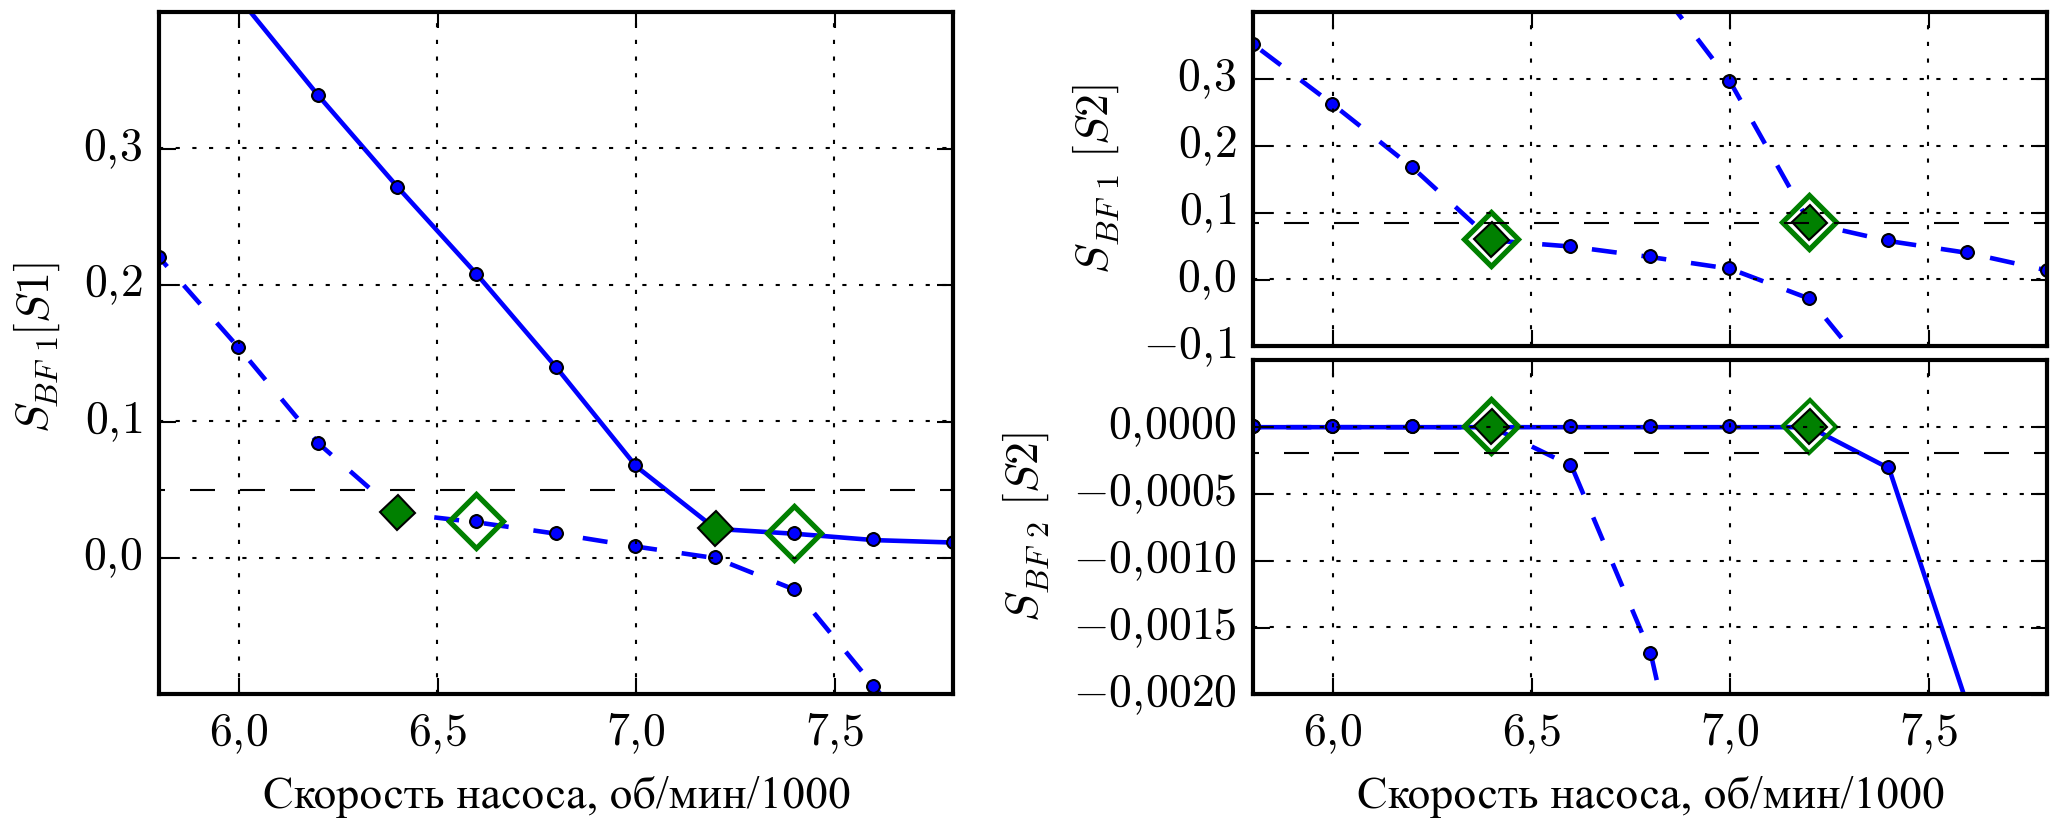
\includegraphics [scale=1.0] {../images/c4_bf}
  \caption{Определение режима обратного течения через насос для роторных насосов крови Спутник 1 (слева) и Спутник 2 (справа) при cF 0,5 (сплошная линия) и cF 0,25 (пунктирная линия)} 
  \label{img:backflow_identification}  
\end{figure}

Пустыми зелеными маркерами отмечен переход между режимами $P_{BF}$ и $P_{PA}$, определенный из зависимости $Q_{P[min]}$ от скорости насоса. 

Малыми зелеными маркерам отмечен переход между режимами $P_{BF}$ и $P_{PA}$, определенных с помощью пороговых значений, которые отмечены пунктирными линиями. Уменьшение индекса ниже порогового значения рассматривалось как переход в режим частичной разгрузки желудочка.

Для определения перехода между режимами обратного течения крови и частичной разгрузки для насоса Спутник 2 предложены два аналогичных индекса, позволяющие определить данный переход с точностью 100\%. 

Пример определения режимов частичной разгрузки и полной разгрузки желудочка сердца для двух поколений роторного насоса крови Спутник представлен на рисунке \ref{img:pa_fa_identification}.

\begin{figure}[H] 
  \center
  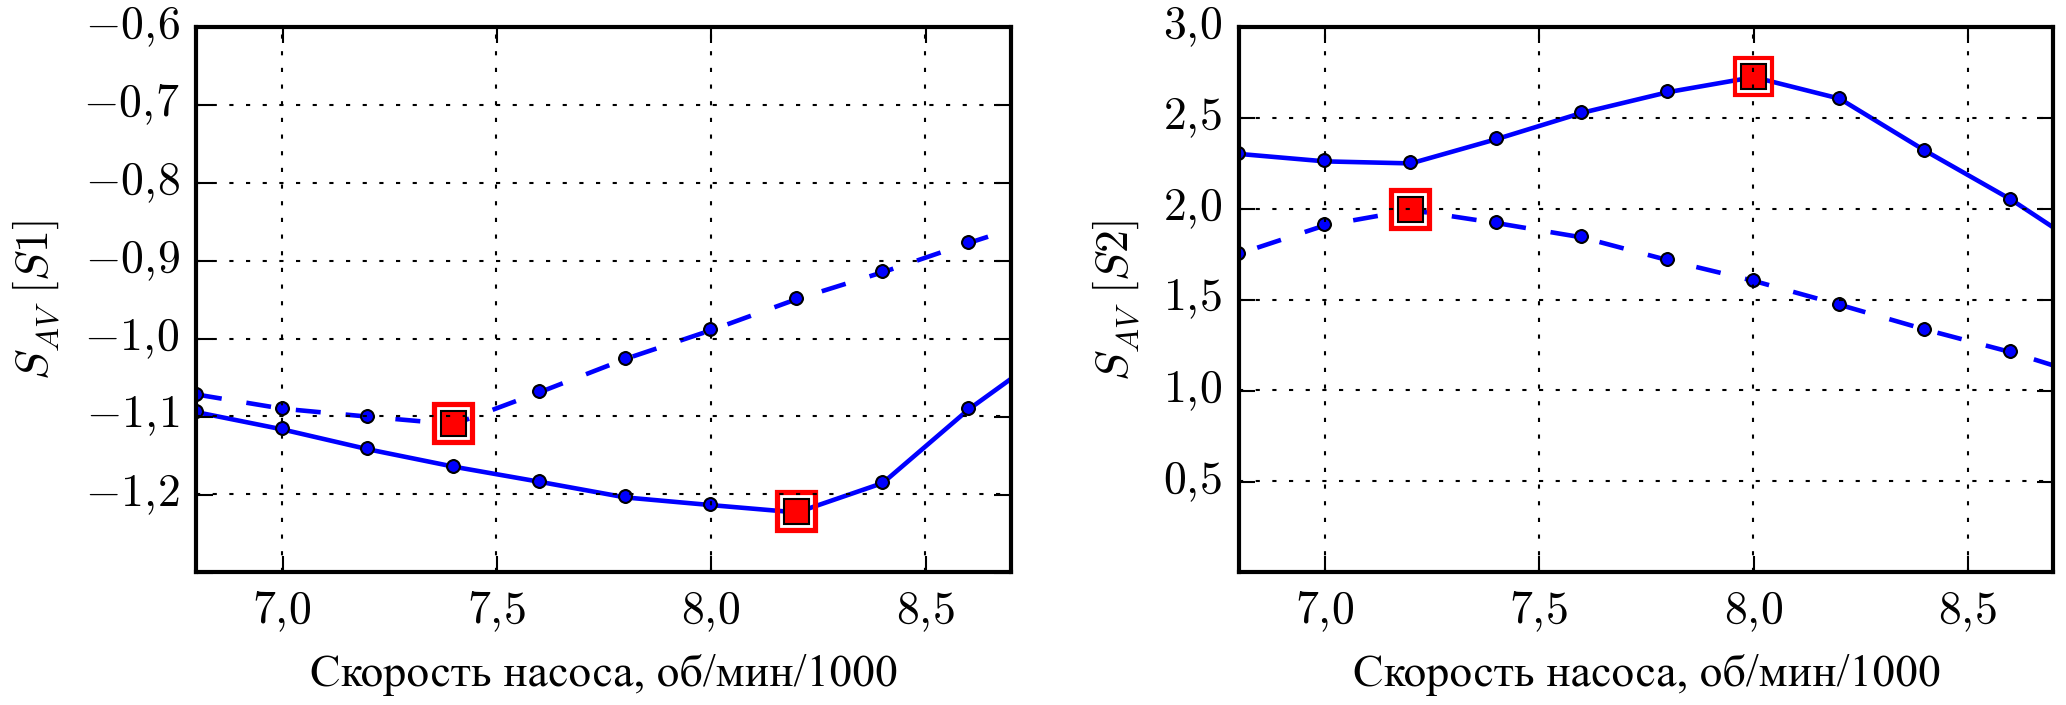
\includegraphics [scale=1.0] {../images/c4_av}
  \caption{Определение режимов частичной разгрузки и полной разгрузки желудочка сердца для роторных насосов крови Спутник 1 (слева) и Спутник 2 (справа) при cF 0,5 (сплошная линия) и cF 0,25 (пунктирная линия)} 
  \label{img:pa_fa_identification}  
\end{figure}

Большим квадратным маркером отмечен переход между режимами $P_{PA}$ и $P_{FA}$, определенный из зависимости $Q_{AV}$ от скорости насоса. Изменение в динамике индекса $S_{AV}$ при увеличении скорости насоса, отмеченное малым красным маркером, позволяет определить переход со 100\% точностью.  

Пример определения режима коллапса желудочка сердца для двух поколений роторного насоса крови Спутник представлен на рисунке \ref{img:collapse_identification}.

\begin{figure}[H] 
  \center
  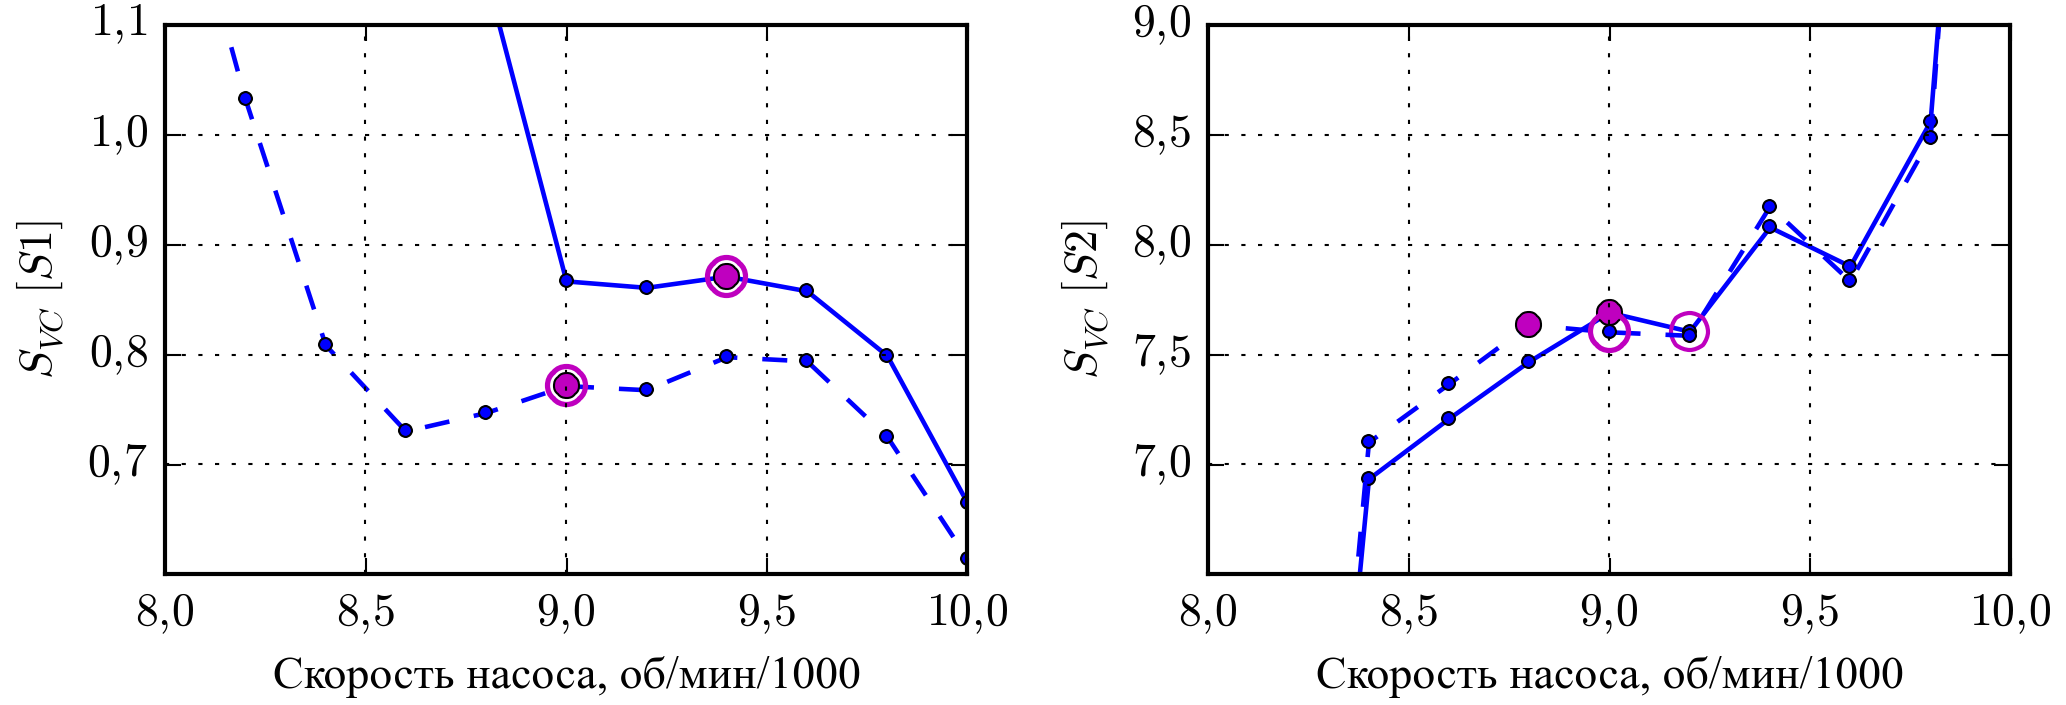
\includegraphics [scale=1.0] {../images/c4_vc}
  \caption{Определение режима коллапса желудочка сердца для роторных насосов крови Спутник 1 (слева) и Спутник 2 (справа) при cF 0,5 (сплошная линия) и cF 0,25 (пунктирная линия)} 
  \label{img:collapse_identification}  
\end{figure}

Большим круглым маркером фиолетового цвета отмечен переход между режимами $P_{FA}$ и $P_{VC}$, определенный из зависимости $P_{ED}$ от скорости насоса. 

Определение перехода к режиму  $P_{VC}$ с помощью индекса возможно со 100\% точностью для роторного насоса крови Спутник 1 и с точностью около 91\% для роторного насоса крови Спутник 2. В каждом случае переход в режим коллапса желудочка сердца определялся как локальный максимум индекса. 

Математические модели имплантируемых роторных насосов крови, описываемые уравнениями \eqref{eq:sputnik_1_eq} и \eqref{eq:sputnik_2_eq}, были исследованы на математической модели сердечно-сосудистой системы, описание которой приводится в разделе \ref{cvs_model_implementation}.
Результаты исследования, аналогичные результатам исследования в испытательном стенде (рисунки \ref{img:ps_sputnik_1} и \ref{img:ps_sputnik_2}) представлены на рисунке \ref{img:cvs_rbp_investigation_c5}.

\begin{figure}[ht]
  \begin{minipage}[ht]{0.49\linewidth}
    \center{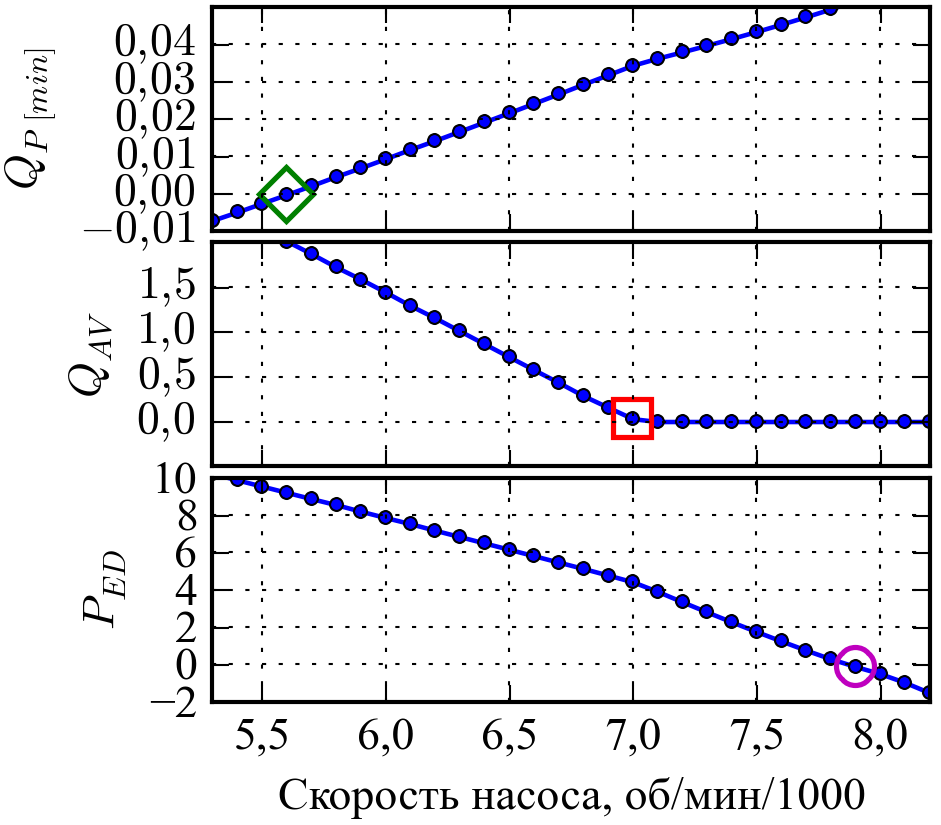
\includegraphics[scale=1.0]{../images/c4_cvs_sputnik_1} \\ а)}
  \end{minipage}
  \hfill
  \begin{minipage}[ht]{0.49\linewidth}
    \center{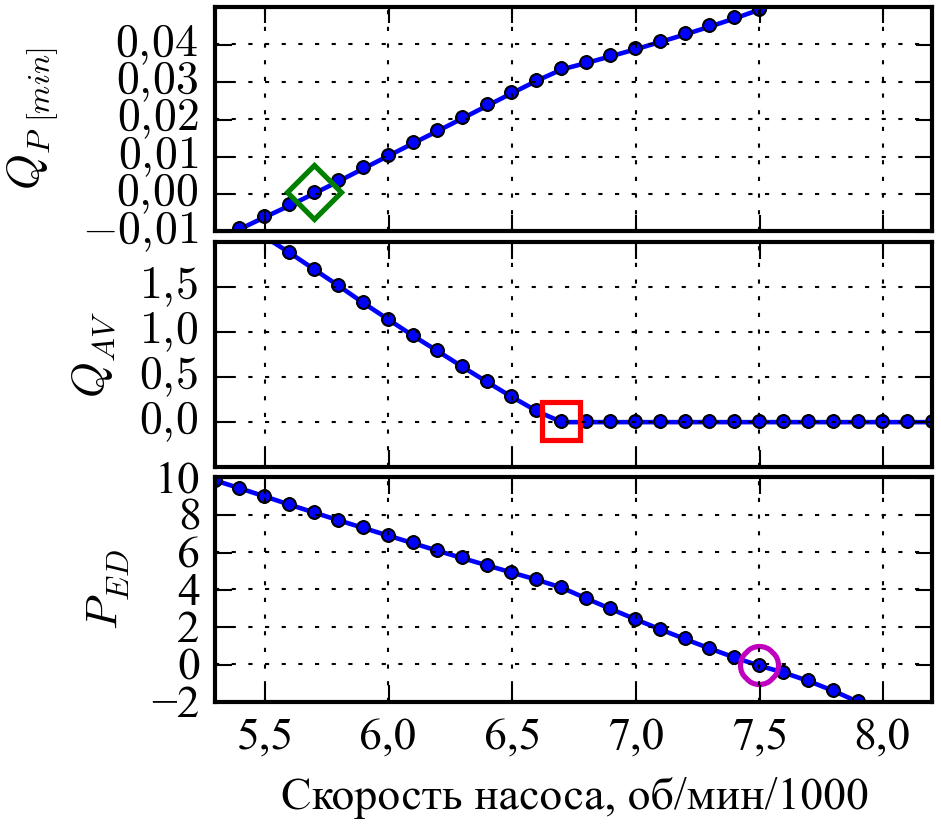
\includegraphics[scale=1.0]{../images/c4_cvs_sputnik_2} \\ б)}
  \end{minipage}
  \caption{Зависимости минимального расхода насоса во время сердечного цикла $Q_{P[min]}$, потока через аортальный клапан $Q_{AV}$ и конечно-диастолического давления желудочка сердца $P_{ED}$ от скорости насоса для роторного насоса крови а) Спутник 1 и б) Спутник 2}
  \label{img:cvs_rbp_investigation_c5}  
\end{figure}

Индексы, приведенные в таблице \ref{tbl:sputnik_indices_and_derivatives}, были исследованы на модели сердечно-сосудистой системы в условиях сердечной недостаточности. Исходная частота сердечных сокращений задана равной 80 уд/мин, исходная сократимость левого желудочка сердца задана с помощью параметра $C_V$ в модели сердца равного 0,5, скорость вращения ротора насоса задана постоянной величиной. 

Точность определения переходов между режимами работы насоса рассчитывалась по формуле \eqref{eq:ps_identification_accuracy}. Значения $\omega_{max}$ и $\omega_{min}$ были определены из зависимостей, представленных на рисунке \ref{img:cvs_rbp_investigation_c5}. Таким образом, $\omega_{max}$ и $\omega_{min}$ для насоса Спутник 1 равнялись 8000 об/мин и 5500 об/мин, для насоса Спутник 2 -- 7600 об/мин и 5600 об/мин соответственно. 

Результаты исследования индексов представлены на рисунках \ref{img:cvs_model_test_s1} и \ref{img:cvs_model_test_s2}.

\begin{figure}[!ht] 
  \center
  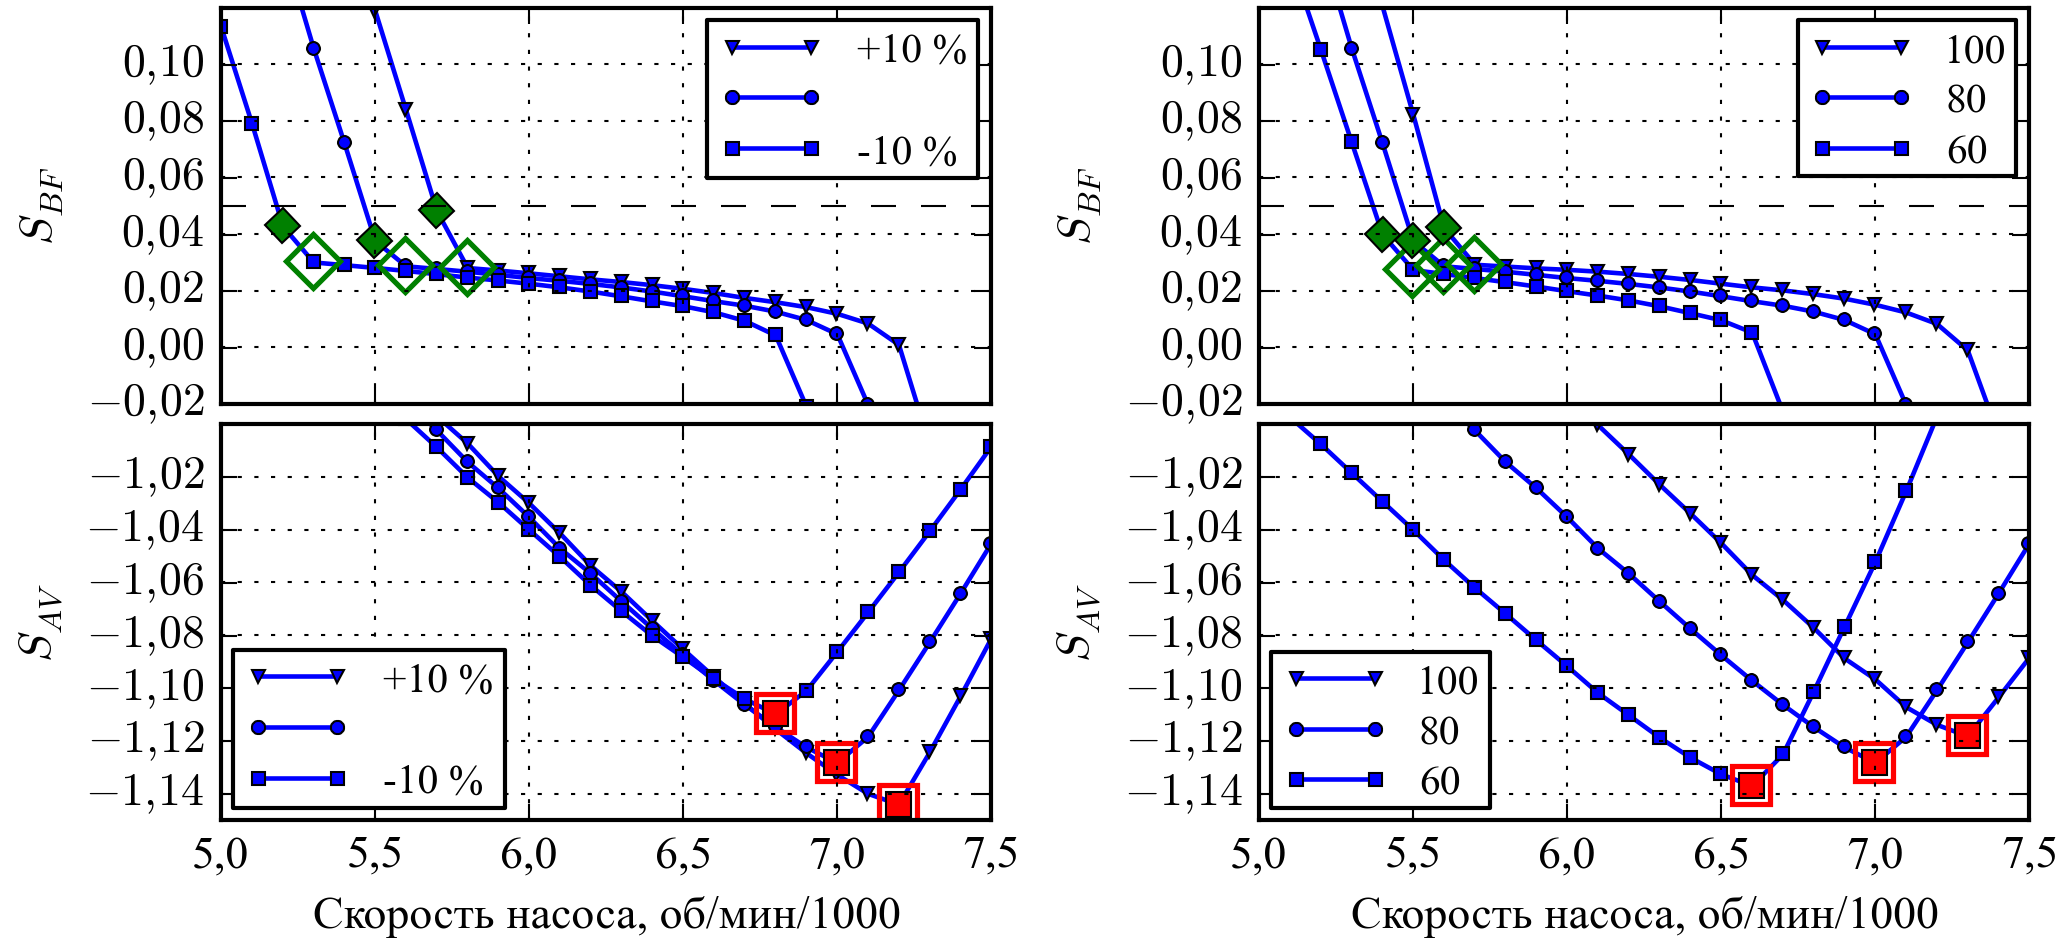
\includegraphics [scale=1.0] {../images/c4_cvs_pumping_states_sputnik_1}
  \caption{Зависимость индексов $S_{BF}$ и $S_{AV}$ от скорости насоса для роторного насоса крови Спутник 1 при изменении сократимости левого желудочка сердца, \% (слева) и частоты сердечных сокращений, уд/мин (справа)} 
  \label{img:cvs_model_test_s1}  
\end{figure}

\begin{figure}[!ht] 
  \center
  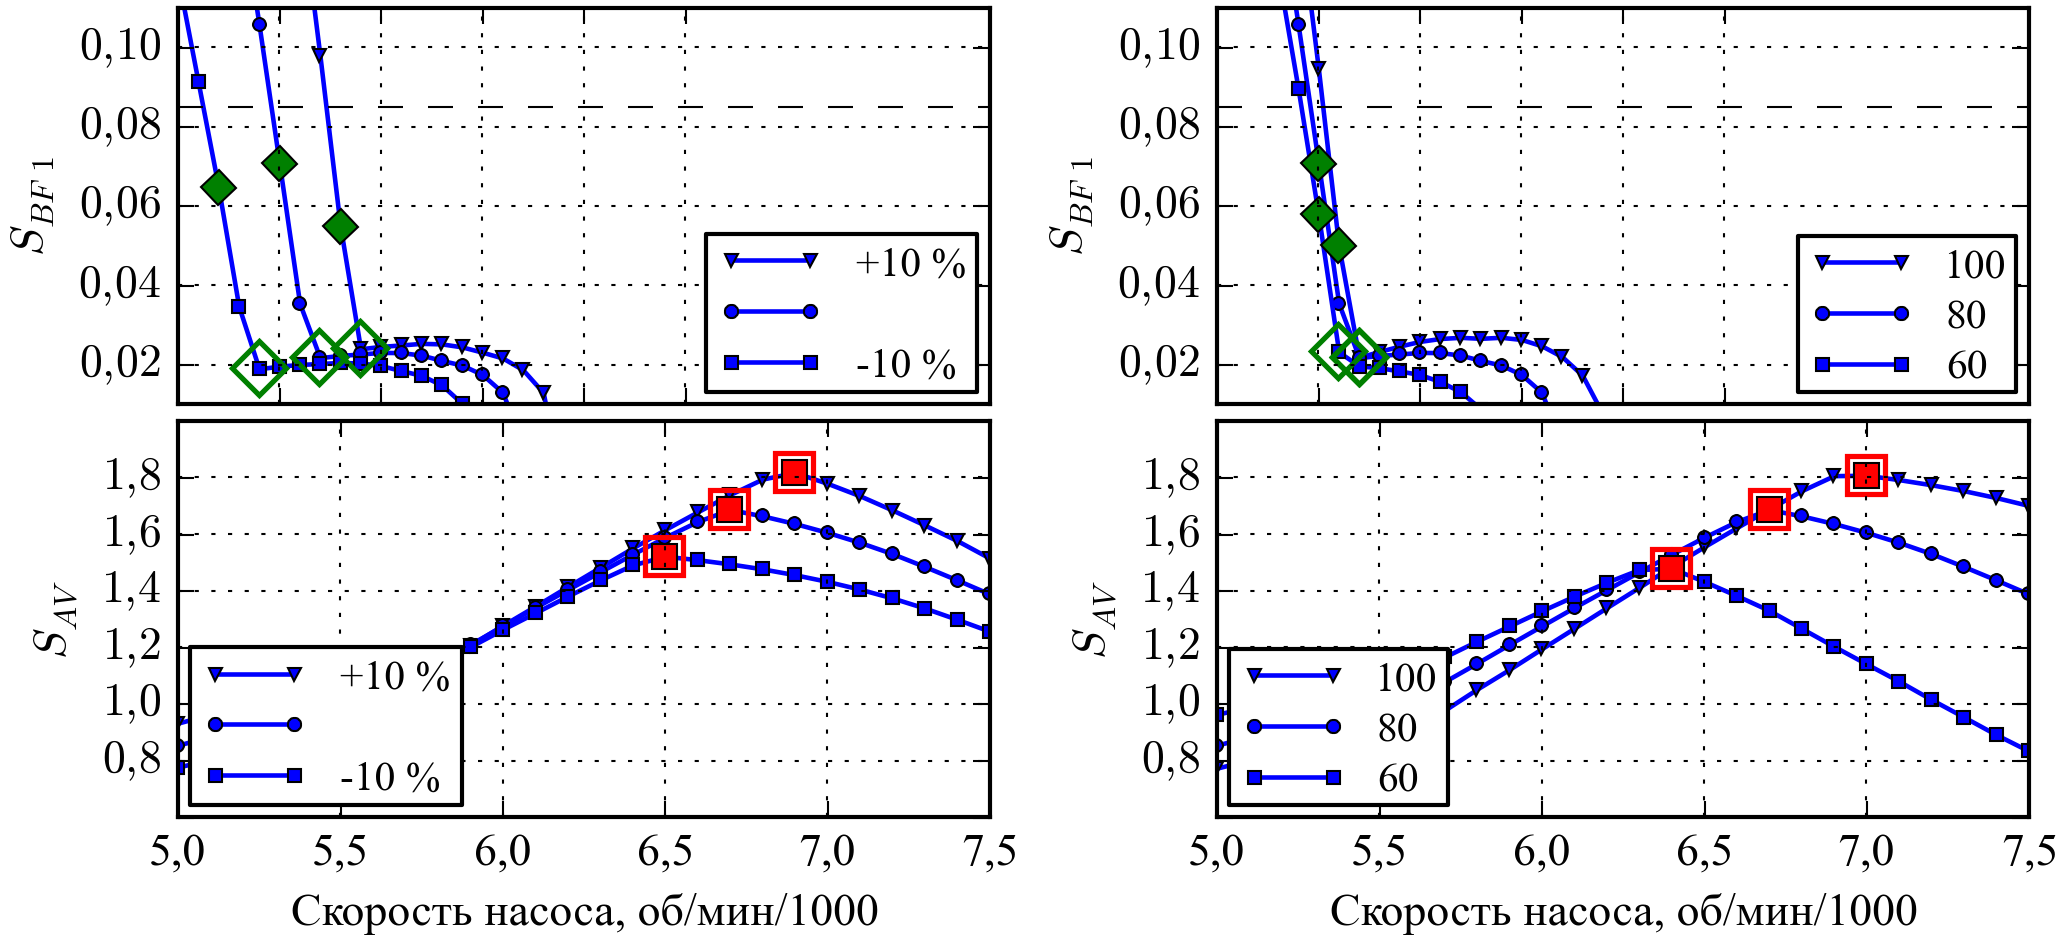
\includegraphics [scale=1.0] {../images/c4_cvs_pumping_states_sputnik_2}
  \caption{Зависимость индексов $S_{BF}$ и $S_{AV}$ от скорости насоса для роторного насоса крови Спутник 2 при изменении сократимости левого желудочка сердца, \% (слева) и частоты сердечных сокращений, уд/мин (справа)} 
  \label{img:cvs_model_test_s2}  
\end{figure}

Результаты расчета точности определения переходов между режимами работы насоса для роторных насосов крови Спутник 1 и Спутник 2 представлены в таблице \ref{tbl:sputnik_ps_cvs}.

\begin{table} [htbp]%
    \centering
	\caption{Точность определения переходов между режимами работы насоса в модели сердечно-сосудистой системы ($\delta(PS)$, \%)}%
	\label{tbl:sputnik_ps_cvs}% label всегда желательно идти после caption
    \renewcommand{\arraystretch}{1.5} 
	\begin{tabular}{@{}@{\extracolsep{20pt}}lllll@{}} 
	\toprule
	& Спутник 1 & & Спутник 2 & \\
	\midrule
	%			&	cF 0,5	& cF 0,25 &	cF 0, & \\
	%\midrule
	$\delta(P_{BF}/P_{PA})$					& 96,0			&		& 92,5		& \\
	$\delta(P_{PA}/P_{FA})$	& 100,0		&		& 100,0		& \\
	\bottomrule
	\end{tabular}%
\end{table}

В результате оказалось возможным определить режимы обратного течения и частичной разгрузки и полной разгрузки желудочка сердца с точностью не менее 92 \%. В ходе исследования индексов установлено, что режим коллапса желудочка не может быть определен, что обусловлено постоянством скорости насоса при моделировании. По этой причине также невозможно использование индекса $S_{BF2}$ для насоса Спутник 2.

%Результаты определения данных режимов для роторного насоса крови Спутник 1

\section*{Выводы по главе 4} 
\addcontentsline{toc}{section}{Выводы по главе 4}

В данной главе проведено исследование взаимодействия имплантируемого роторного насоса крови и сердечно-сосудистой системы с использованием экспериментальных данных, полученных в испытательном гидродинамическом стенде для двух поколений имплантируемого роторного насоса крови Спутник.

В ходе исследования заданы следующие пороговые величины для критериев оценки эффективности идентификации: средняя точность оценки расхода насоса не менее 90\% и точность определения переходов между режимами работы насоса не менее 80\%.

Установлено несоответствие заданным пороговым величинам в случае использования математической модели, описываемой уравнением \eqref{eq:final_pump_model} -- средняя точность оценки расхода составила менее 90\%, точность определения перехода $P_{BF}/P_{PA}$ -- менее 70\% и точность определения перехода $P_{FA}/P_{VC}$ -- не более 75\%.

Данная проблема была решена посредством построения математических моделей имплантируемых роторных насосов крови Спутник с использованием алгоритма структурно-параметрической идентификации, разработанного во \ref{chapt2}-й главе. В результате были построены математические модели, которые обеспечивают среднюю точность оценки расхода насоса не менее 90\% и точность определения переходов между режимами работы насоса более 91\%, что соответствует заданным пороговым величинам для критериев оценки эффективности идентификации. 

В результате исследования построенных математических моделей на модели сердечно-сосудистой системы при изменении сократимости желудочка сердца и частоты сердечных сокращений продемонстрирована возможность определения переходов $P_{BF}/P_{PA}$ и $P_{PA}/P_{FA}$ с точностью не менее 92\%. Определение режима коллапса желудочка сердца $P_{VC}$ оказалась невозможным из-за постоянства скорости вращения ротора при моделировании.    

% Результаты, демонстрирующие возможности управления имплантируемым роторным насосом крови Спутник 1 на модели сердечно-сосудистой системы с использованием полученных экспериментальных данных, опубликованы в работе \cite{mt6_2016}. 

Полученные результаты могут быть использованы для управления имплантируемыми роторными насосами крови при проведении экспериментальных исследований в испытательных гидродинамических стендах. 

% Отслеживание изменений производных также похоже на подход, используемый в работе \cite{Hui_2014}, где сообщается что градиентные индексы наиболее точны при определении закрытого состояния АК. Тем не менее, мы полагаем, что данный подход оправдан по следующим соображением: необходимость точной оценки расхода в динамических условиях, определение множества режимов работы и возможность использования в качестве средства диагностики (т.\:е. представляет собой основу для системы адаптивного управления роторными насосами крови в рамках существующей технологии). Кроме того, данный метод заключается не только в анализе временных диаграмм сигналов насоса, а в генерации различных вариантов сигналов, описывающих динамику течения крови через насос и изменяющихся согласованно с изменениями этой динамики. Он также позволяет расширить возможности алгоритмов, которые используют индексы на основе временных диаграмм сигналов насоса, поскольку с необходимостью предоставляют новые варианты сигналов, которые обусловлены или 
% связаны с работой насоса в динамических условиях.
% 
% Результаты моделирования на сердечно-сосудистой системе показывают, что индексы для определения коллапса не позволяют определить данное состояние из-за постоянства скорости в случае математического моделирования. Мы предполагаем, что успех алгоритмов, определяющих данное состояние из временной диаграммы скорости насоса, таких как \cite{4463021, Ng_2013}, обусловлен пульсирующей компонентой скорости, образующейся благодаря сокращениям сердца, т.\:е. состояние данного типа в наибольшей степени влияет на данный сигнал.
% 
% В тоже время, можно предполагать, что изменение других неинвазивно измеренных сигналов насоса, такие как электрический ток двигателя или противо-ЭДС, в большей степени будет связано с либо с обратным течением крови через насос, функциональностью аортального клапана и т.\:д. 
% 
